
\begin{myex}
	
	\textbf{Nombre d'enfants par maison dans un lotissement}
	
	\begin{multicols*}{2}
		
		\begin{center}
			\begin{tabular}{|@{\ }c@{\ }|@{\ }c@{\ }|}
				\hline
				Nombre d'enfants & Nombre de maison \\ \hline
				0 & 3  \\ \hline
				1 & 12 \\ \hline
				2 & 9 \\ \hline
				3 & 6 \\ \hline
			\end{tabular}
		\end{center}
		
		
		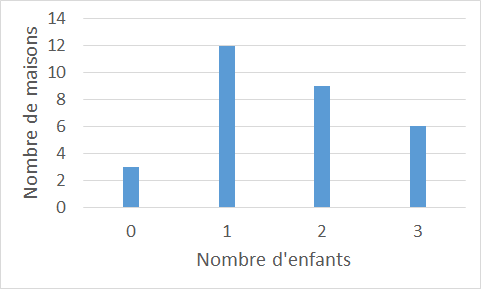
\includegraphics[scale=0.8]{img/barres}
	\end{multicols*}
	
\end{myex}

